\documentclass[../nirs.tex]{subfiles}
\usepackage{rotating}

\begin{document}
\section{Выявление основных понятий и процессов, их свойств и закономерностей.
Построение ER-диаграммы предметной области}

\subsection{Основные понятия}
Путевой лист -- это документ для учёта и контроля работы водителя и
транспортного средства (п. 14 ст. 2 Федерального закона от 08.11.2007 № 259-ФЗ).
В нём прописывается маршрут и техническое состояние машины, информация о
проведённом медосмотре водителя и пр. Путевые листы нужны, чтобы обосновать
необходимость аренды или лизинга, а также подтвердить расходы, связанные с
использованием транспортных средств. Путевые листы составляют индивидуальные
предприниматели и организации всех форм собственности, которые используют
транспорт в своей деятельности или для собственных нужд [3].

Горюче-смазочные материалы (ГСМ) -- общее обозначение широкого спектра веществ,
обеспечивающих бесперебойную работу двигателей внутреннего сгорания и различных
технических узлов. Они включают смазочные материалы, горючее и технические
жидкости [4].

Техническое обслуживание -- это комплекс организационно-технических мероприятий
и работ, производимых на объекте и направленных на поддержание в рабочем или
исправном состоянии оборудования (программного обеспечения) технических систем в
процессе их использования по назначению, с целью повышения надежности и
эффективности их работы [5].

\subsection{Основные процессы}
Заключение договора -- во время которого рассматривается заказ на оказание
транспортных услуг, определяется необходимое для его выполнения количество
единиц техники, устанавливается цена за оказание транспортных услуг, а также
заключение договора с клиентом.

Выпуск техники -- процесс составления разнарядки, в соответствии с заявками
клиентов, выдача путевых листов водителям автотранспорта, предрейсовый контроль
технического состояния транспорта, выдача ГСМ выпущенной на линию техники.

Сервис и ремонт -- отвечает за календарное планирование графика прохождения
технического обслуживания транспортной техники, передача ее в сервис и
возвращение из него.

Документооборот -- процесс обработки путевых листов, с целью списания
горюче-смазочных средств, а также расчета работы техники за смену.

\subsection{Построение ER-диаграммы предметной области}
Классовая диаграмма разрабатываемой системы представлена на рисунке
\ref{fig:2_1_3_er_diagram}.

\begin{figure}[hp!]
	\centering
	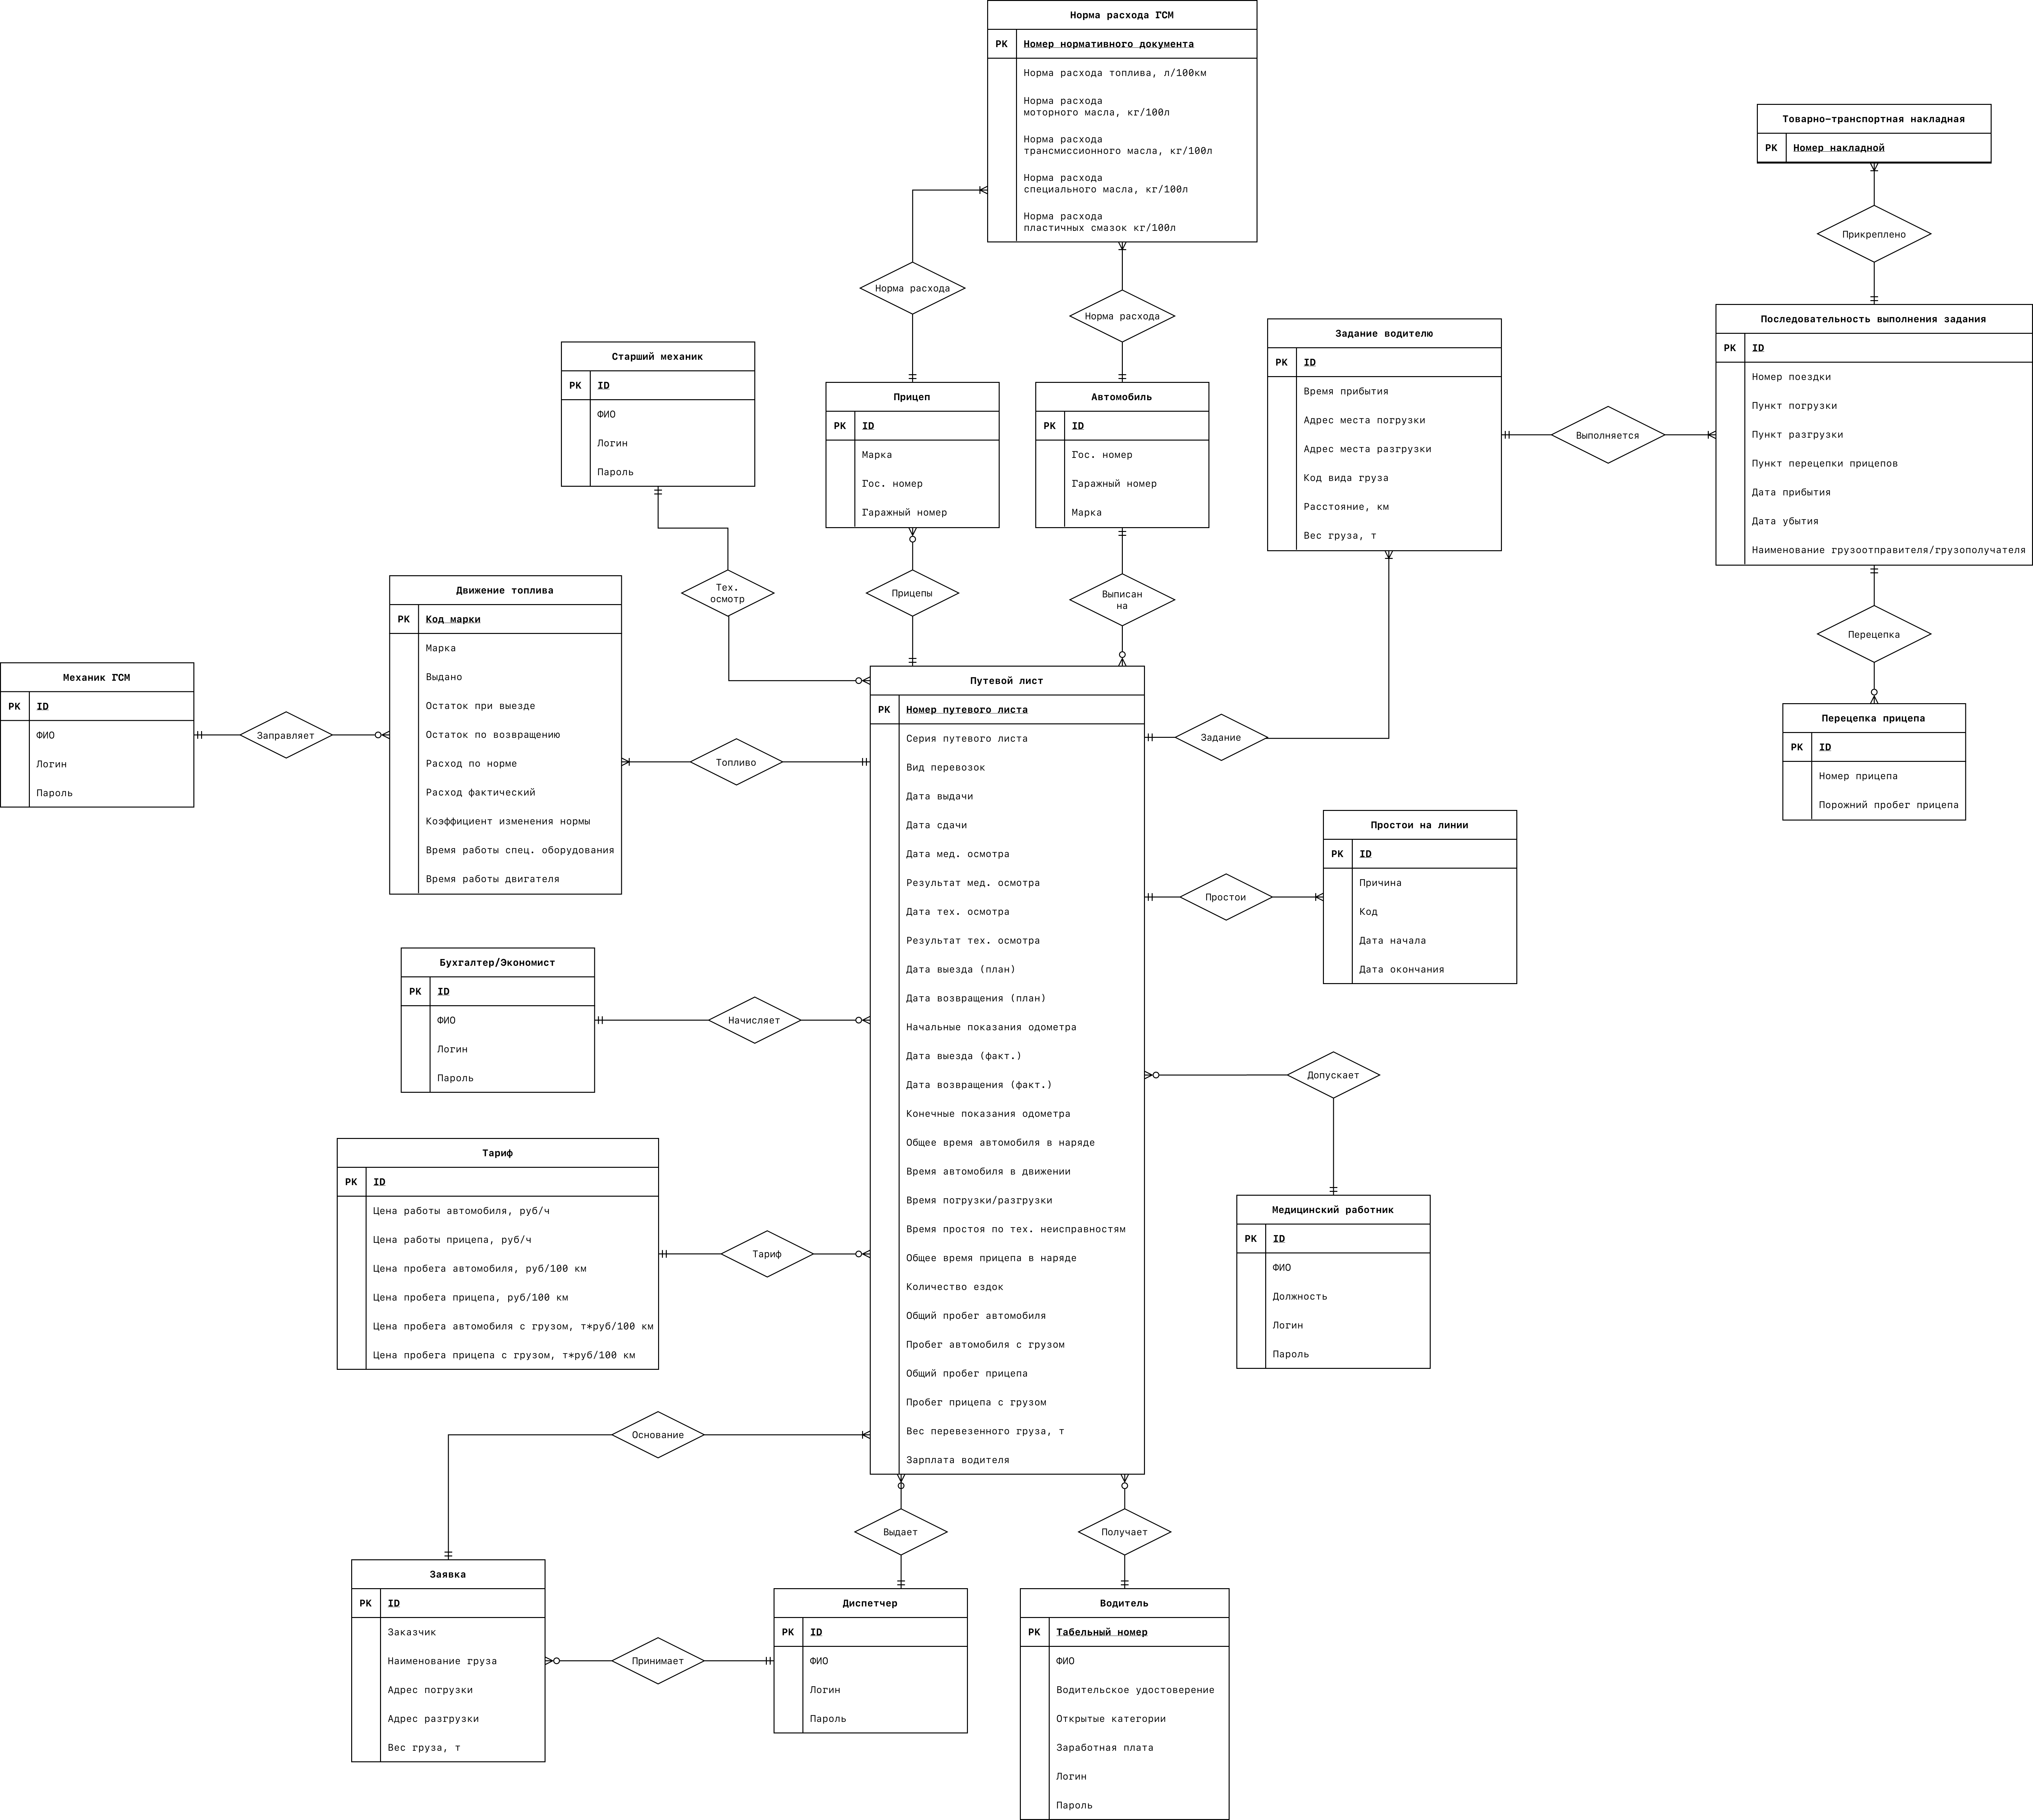
\includegraphics[keepaspectratio,width=\textwidth]{./images/2_1_3_er-diagram.png}
	\caption{ER-диаграмма системы}
	\label{fig:2_1_3_er_diagram}
\end{figure}

Центральной сущностью выступает \textquote{Путевой лист}. Она является
электронным аналогом путевого листа, заполняющегося на бумажном носителе.
Путевые листы формируются на основе заявок от заказчиков.

Диспетчер принимает заявку на предоставление транспортных услуг и выписывает на
ее основании путевые листы на каждую единицу техники, требующуюся для выполнения
данной заявки. На основании заявки заказчика диспетчер формирует задание
водителю. Здесь указываются время подачи техники на место погрузки, адрес места
погрузки и разгрузки, код вида груза, вес груза и расстояние между пунктами
погрузки и разгрузки.

Во время выполнения задания, водитель заполняет последовательность выполнения
задания. В ней указывается порядковый номер поездки; адреса пункта погрузки,
пункта разгрузки, и, при необходимости, пункта перецепки прицепов; даты убытия с
места погрузки и прибытия на пункт разгрузки; наименование грузоотправителя
и/или грузополучателя. Для подтверждения факта транспортировки груза в путевом
листе прикладываются номера товарно-транспортных накладных на перевозимые грузы.

Старший механик проводит технический осмотр техники, с целью выявления ее
технического состояния. Заключение о техническом состоянии техники
вносится в путевой лист. При необходимости проведения технических работ
автомобиль отправляют в сервис. Перед выпуском автомобиля из гаража, а также по
его возвращении со смены старший механик проверяет и фиксирует показания
одометра в путевом листе.

Медицинский работник проводит медицинский осмотр водителя, назначенного на
выполнение задания. Результат осмотра фиксируется в путевом листе.

Механик ГСМ проверяет уровень топлива в автомобиле перед его выездом из гаража и
по возвращению со смены. В случае необходимости, заправляет автомобиль.
Количество залитого топлива фиксируется в путевом листе.

По закрытию путевого листа бухгалтер/экономист рассчитывает заработную плату
водителя, списывает израсходованные водителем ГСМ, а также рассчитывает
стоимость оказанных услуг, с учетом действующих на предприятии тарифов.

\end{document}
